\documentclass{article}

\usepackage{graphicx}
\usepackage{tikz}
\usepackage{tikzsymbols}
\usetikzlibrary{calc,patterns,shapes.geometric}
\pagestyle{empty}
\usepackage[margin=0pt]{geometry}
\geometry{papersize={14in,12in}}

\def\centerarc[#1](#2)(#3:#4:#5){\draw[#1] ($(#2)+({#5*cos(#3)},{#5*sin(#3)})$) arc (#3:#4:#5);}

\begin{document}
	\begin{figure}
		\centering
		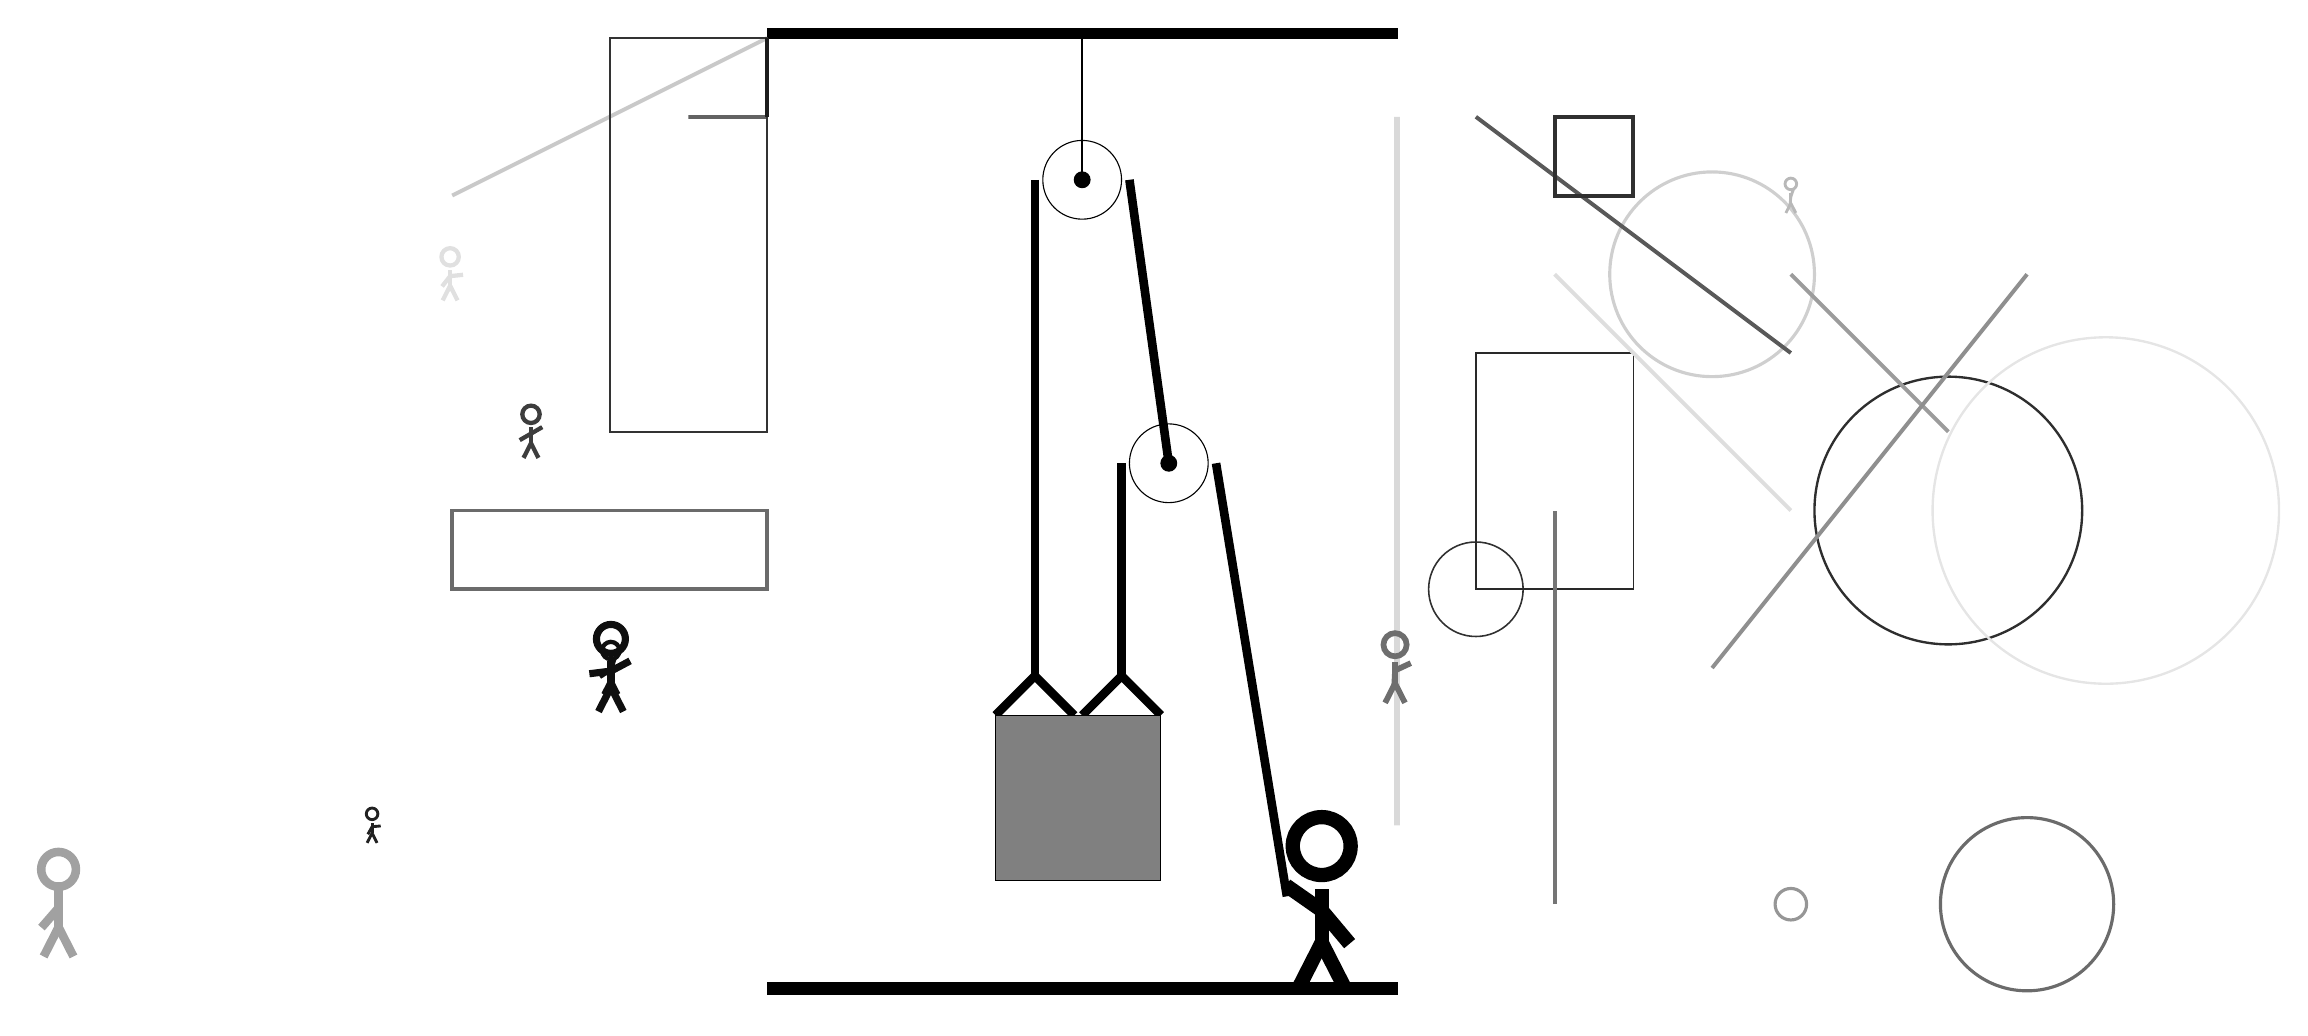
\begin{tikzpicture}
			%%%%% START %%%%%
			
			\draw[fill=black] (-2, 9) rectangle (6, 9.125);
			
			\draw (2, 7.2) circle (0.5);
			\draw[fill=black] (2, 7.2) circle (0.1);
			\draw[thick] (2, 7.2) -- (2, 9);
			
			\draw (3.1, 3.6) circle (0.5);
			\draw[fill=black] (3.1, 3.6) circle (0.1);
			
			\draw[line width = 1.1mm]  (0.9, 0.4) -- (1.4, 0.9) -- (1.9, 0.4);
			\draw[line width = 1.1mm]  (2.0, 0.4) -- (2.5, 0.9) -- (3.0, 0.4);
			\draw[fill=black!50] (0.9, 0.4) rectangle (3.0, -1.7);
			
			\draw[line width=0.7mm, color=black!15] (6, -1) rectangle (6, 8);
			
			\draw [line width=0.4mm, color=black!19](10, 6) circle (1.3);
			\draw[line width=0.5mm, color=black!65](7, 8) -- (11, 5);
			\draw [line width=0.2mm, color=black!81](7, 2) circle (0.6);
			
			\draw[line width=0.5mm, color=black!61] (-3, 8) rectangle (-2, 8);
			\node[line width=0.7mm, color=black!94] at (-4, 1) {\Strichmaxerl[5][7][28]};
			\draw[line width=0.5mm, color=black!21](-6, 7) -- (-2, 9);
			\node[line width=0.5mm, color=black!12] at (-6, 6) {\Strichmaxerl[3][52][6]};
			\draw [line width=0.3mm, color=black!82](13, 3) circle (1.7);
			
			\draw[line width=0.2mm, color=black!84] (7, 2) rectangle (9, 5);
			\draw[line width=0.5mm, color=black!54](8, -2) -- (8, 3);
			\draw[line width=0.5mm, color=black!81] (8, 7) rectangle (9, 8);
			\node[line width=0.3mm, color=black!57] at (6, 1) {\Strichmaxerl[4][87][25]};
			
			\node[line width=0.2mm, color=black!37] at (-11, -2) {\Strichmaxerl[6][49][90]};
			\node[line width=0.3mm, color=black!76] at (-5, 4) {\Strichmaxerl[3][30][30]};
			\draw[line width=0.5mm, color=black!58] (-2, 2) rectangle (-6, 3);
			\draw[line width=0.5mm, color=black!39](11, 6) -- (13, 4);
			\node[line width=0.5mm, color=black!87] at (-7, -1) {\Strichmaxerl[2][61][5]};
			\draw [line width=0.4mm, color=black!58](14, -2) circle (1.1);
			\draw[line width=0.5mm, color=black!44](10, 1) -- (14, 6);
			\draw[line width=0.2mm, color=black!80] (-4, 9) rectangle (-2, 4);
			
			\draw[line width=0.5mm, color=black!89] (-2, 8) rectangle (-2, 9);
			
			\node[line width=0.4mm, color=black!94] at (-4, 1) {\Strichmaxerl[3][33][72]};
			\draw [line width=0.4mm, color=black!41](11, -2) circle (0.2);
			\draw[line width=0.5mm, color=black!98] (7, 3) rectangle (7, 3);
			
			\draw[line width=0.5mm, color=black!13](8, 6) -- (11, 3);
			\draw [line width=0.3mm, color=black!10](15, 3) circle (2.2);
			\node[line width=0.7mm, color=black!28] at (11, 7) {\Strichmaxerl[2][84][71]};
			
			
			\draw[line width = 1.1mm] (1.4, 7.2) -- (1.4, 0.9);
			\centerarc[line width = 1.1mm](2, 7.2)(0:180:0.6);
			\draw[line width = 1.1mm] (2.6, 7.2) -- (3.1, 3.6);
			\draw[line width = 1.1mm] (2.5, 3.6) -- (2.5, 0.9);
			\centerarc[line width = 1.1mm](3.1, 3.6)(0:180:0.6);
			\draw[line width = 1.1mm] (3.7, 3.6) -- (4.6, -1.9);
			
			\node at (5, -2) {\Strichmaxerl[10][-35][-50]};
			
			\draw[fill=black] (-2, -3) rectangle (6, -3.15);
			
			%%%%% END %%%%%
		\end{tikzpicture}
	\end{figure}	
\end{document}